\documentclass[12pt]{article}
\usepackage[english]{babel}
\usepackage{hyperref}
\usepackage{makeidx}
\usepackage{pgfplots}
\usepackage[a4paper, inner=1.5cm, outer=3cm, top=2cm,bottom=3cm, bindingoffset=1cm]{geometry}
\usepackage{chngcntr}
\counterwithin*{section}{part}
\usepackage{tikz}
\usetikzlibrary{arrows.meta}
\tikzset{%
  >={Latex[width=2mm,length=2mm]},
  % Specifications for style of nodes:
            base/.style = {rectangle, rounded corners, draw=black,
                           minimum width=4cm, minimum height=1cm,
                           text centered, font=\sffamily},
  activityStarts/.style = {base, fill=blue!30},
       startstop/.style = {base, fill=red!30},
    activityRuns/.style = {base, fill=green!30},
         process/.style = {base, minimum width=2.5cm, fill=orange!15,
                           font=\ttfamily},
}
\begin{document}
\begin{titlepage}
    \begin{center}
        \vspace*{1cm} 
        \Huge
        \textbf{Machine Learning in Healthcare} 
        \vspace{0.5cm}
        \normalsize
        \vspace{0cm}
        \\
        Study of machine learning algorithms and application on the Pima Indians Diabetes Dataset.
 
        \vspace{1.5cm}
 
        \textbf{Alexander Roque Rodrigues}
 
        \vfill
 
        A dissertation presented for the degree of\\
        Bachelor in Computer Science
 
        \vspace{0.8cm}
  
        \Large
        Department of Computer Science\\        
        Smt. Parvatibai Chowgule College of Arts and Science\\
        India\\
        18 August 2019
 
    \end{center}
\end{titlepage}
\Huge
\newpage
\huge
\textbf{Acknowledgements}
\normalsize
\newpage
\tableofcontents
\newpage
\part{Background}
Data is everywhere. International initiatives coupled with global disruptive innovation are the leading causes for pushing datafincation forward.

\textbf{Datafication refers to the modern-day trend of digitalizing (or datafying) every aspect of life.}

This data creation is enabling the transformation of data into new and potentially valuable forms. Entire municipalities are being incentivized to become smarter. In the not too
distant future, our towns and cities will collect thousands of variables in
real time to optimize, maintain, and enhance the quality of life for entire
populations. One would reasonably expect that as well as managing traffic,
traffic lights may also collect other data such as air quality, visibility, and
speed of traffic. As a result of big data from connected devices, embedded
sensors, and the IoT, there is a global need for the analysis, interpretation,
and visualization of data.

\newpage
\section{Diabetes Mellitus}
More commonly referred to as "diabetes" -- a chronic disease associated with abnormally high levels of the sugar glucose in the blood. Diabetes is due to one of two mechanisms:

Inadequate production of insulin (which is made by the pancreas and lowers blood glucose), or
Inadequate sensitivity of cells to the action of insulin.
The two main types of diabetes correspond to these two mechanisms and are called insulin dependent (type 1) and non-insulin dependent (type 2) diabetes. In type 1 diabetes there is no insulin or not enough of it. In type 2 diabetes, there is generally enough insulin but the cells upon which it should act are not normally sensitive to its action.

The signs and symptoms of both types of diabetes include increased urine output and decreased appetite as well as fatigue. Diabetes is diagnosed by blood glucose testing, the glucose tolerance test, and testing of the level of glycosylated hemoglobin (glycohemoglobin or hemoglobin A1C). The mode of treatment depends on the type of the diabetes.

The major complications of diabetes include dangerously elevated blood sugar, abnormally low blood sugar due to diabetes medications, and disease of the blood vessels which can damage the eyes, kidneys, nerves, and heart.

\newpage
\part{Review of Literature}
\section{Predicting Diabetes Mellitus With Machine Learning Techniques}
Diabetes is segregated into 2 categories 
\newpage
\part{Data Preprocessing}
\section{Feature Extraction}
\subsection{Filters}
\subsection{Wrappers}
\newpage
\part{Machine Learning Algorithms}
\newpage
\section{Linear Regression}
\subsection{Introduction to Linear Regression}
Linear regression is a forecasting technique that can be use to predict the future of a number series based on the historic data given. The perks of using a linear regression model are as follows:

\begin{itemize}
  \item produces decent and  easy to interpret results.
  \item is computationally inexpensive.
  \item conversion of algorithm into code does not take much effort or time.
  \item numeric values as well as nominal values support is offered.
\end{itemize}

However, a major drawback of linear regression is that it \textbf{poorly models nonlinear data}.
\\
Considering a dataset that has values ranging from 
$X = \lbrace x_{1}+x_{2}+x_{3}+...+x_{n} \rbrace$ where
all the entries of the dataset are real numbers. Each $x_{i}$ is associated with a corresponding value of $y_{i}$ from the dataset $Y = \lbrace y_{1}+y_{2}+y_{3}+...+y_{n} \rbrace$.

The most basic equation for linear regression can be expressed via this simple equation.
$$y = \beta_{0}x+\beta_{1}+\epsilon$$

So to minimize the error in the predictions, a way to calculate the error should be formulated. A loss function in machine learning is simply a measure of how different the predicted value is from the actual value. The Quadratic Loss Function to calculate the loss or error in our linear regression model. It can be defined as:
$$L(x) = \sum_{i=1}^{n}(y_{i}-p_{i})^{2} $$
Therefore using the method of Least Squares, we can find the values of $\beta_{0}$ and $\beta_{1}$.

$$
\beta_{0} = \frac{\sum_{i=1}^{n} ( x_{i}-\bar{x}) (y_{i}-\bar{y})}{\sum_{i=1}^{n} ( x_{i}-\bar{x})^{2} }
$$
The linear regression model with an error value close to 1.00 indicates a perfect model and those with values closer to 0.00 indicates a model that delivers poor performance.

\newpage
\section{Logistic Regression}
Even if called regression, this is a classification method which is based on the probability for
a sample to belong to a class. As our probabilities must be continuous in R and bounded
between (0, 1), it's necessary to introduce a threshold function to filter the term z. The name
logistic comes from the decision to use the sigmoid (or logistic) function:
% page 97 sigmoid formula

\newpage
\section{K-Nearest Neighbours}
The k-means algorithm is based on the (strong) initial condition to decide the number of
clusters through the assignment of k initial centroids or means:
% page 183
\\
Then the distance between each sample and each centroid is computed and the sample is
assigned to the cluster where the distance is minimum. This approach is often called
minimizing the inertia of the clusters, which is defined as follows:
%page 183
\\
The process is iterative—once all the samples have been processed, a new set of centroids
K (1) is computed (now considering the actual elements belonging to the cluster), and all the
distances are recomputed. The algorithm stops when the desired tolerance is reached, or in
other words, when the centroids become stable and, therefore, the inertia is minimized.
Of course, this approach is quite sensitive to the initial conditions, and some methods have
been studied to improve the convergence speed. One of them is called k-means++ (Karteeka
Pavan K., Allam Appa Rao, Dattatreya Rao A. V., and Sridhar G.R., Robust Seed Selection
Algorithm for K-Means Type Algorithms, International Journal of Computer Science and
Information Technology 3, no. 5, October 30, 2011), which selects the initial centroids so that
they are statistically close to the final ones. The mathematical explanation is quite difficult;
however, this method is the default choice for scikit-learn, and it's normally the best choice
for any clustering problem solvable with this algorithm.
% page 188
\subsection{Finding Optimum Number of Clusters}
One of the most common disadvantages of k-means is related to the choice of the optimal
number of clusters. An excessively small value will determine large groupings that contain
heterogeneous elements, while a large number leads to a scenario where it can be difficult
to identify the differences among clusters. Therefore, we're going to discuss some methods
that can be employed to determine the appropriate number of splits and to evaluate the
corresponding performance.

\newpage
\section{Decision Tree}

\newpage
\section{Random Forest}

\newpage
\section{Gradient Boosting}

\newpage
\section{Support Vector Machine}
Support Vector Machines is an algorithm that is capable of handling 
linear as well as data that occurs non-linearly. For example, for a long time, SVMs were the best
choice for MNIST dataset classification, thanks to the fact that they can capture very high
non-linear dynamics using a mathematical trick, without complex modifications in the
algorithm.

\subsection{Linear Support Vector Machines}
Let us consider a dataset of features we want to classify.

$$
X = \lbrace x_{1}, x_{2}, x_{3}, ... , x_{n} \rbrace 
$$ For the target variable, we will consider the dataset $Y$, with target outcomes as $\lbrace0,1\rbrace$ indicating a true or false condition.

$$
Y = \lbrace y_{1}, y_{2}, y_{3}, ... , y_{n} \rbrace 
$$

\newpage
\section{Perceptron}
The perceptron is the foundation of neural networks.

\newpage
\section{Multilayered Perceptron}

\newpage
\part{Real World Application}

\newpage
\part{Building Information Systems for Prediction}
\section{Introduction}
In today's world we have many algorithms and multiple datasets along with sufficient data available for testing and training the algorithms.



\section{Feature Selection}
\newpage
\section{Models}
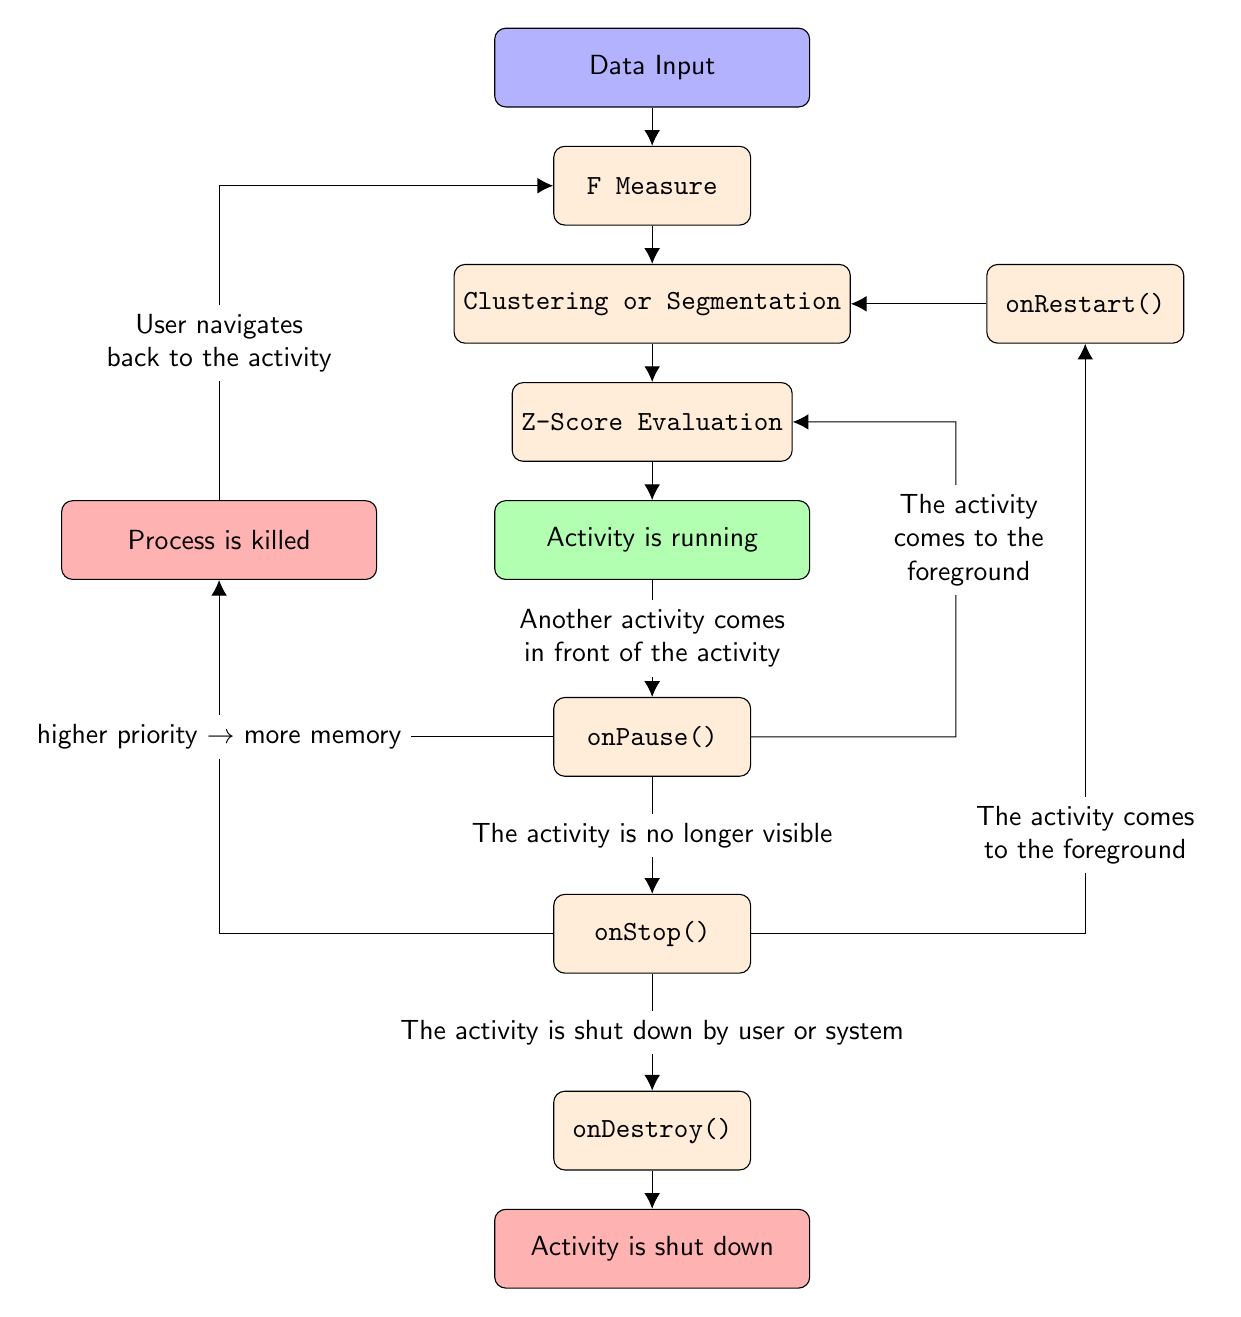
\begin{tikzpicture}[node distance=1.5cm,
    every node/.style={fill=white, font=\sffamily}, align=center]
  % Specification of nodes (position, etc.)
  \node (start)             [activityStarts]              {Data Input};
  \node (onCreateBlock)     [process, below of=start]          {F Measure};
  \node (onStartBlock)      [process, below of=onCreateBlock]   {Clustering or Segmentation};
  \node (onResumeBlock)     [process, below of=onStartBlock]   {Z-Score Evaluation};
  \node (activityRuns)      [activityRuns, below of=onResumeBlock]
                                                      {Activity is running};
  \node (onPauseBlock)      [process, below of=activityRuns, yshift=-1cm]
                                                                {onPause()};
  \node (onStopBlock)       [process, below of=onPauseBlock, yshift=-1cm]
                                                                 {onStop()};
  \node (onDestroyBlock)    [process, below of=onStopBlock, yshift=-1cm] 
                                                              {onDestroy()};
  \node (onRestartBlock)    [process, right of=onStartBlock, xshift=4cm]
                                                              {onRestart()};
  \node (ActivityEnds)      [startstop, left of=activityRuns, xshift=-4cm]
                                                        {Process is killed};
  \node (ActivityDestroyed) [startstop, below of=onDestroyBlock]
                                                    {Activity is shut down};     
  % Specification of lines between nodes specified above
  % with aditional nodes for description 
  \draw[->]             (start) -- (onCreateBlock);
  \draw[->]     (onCreateBlock) -- (onStartBlock);
  \draw[->]      (onStartBlock) -- (onResumeBlock);
  \draw[->]     (onResumeBlock) -- (activityRuns);
  \draw[->]      (activityRuns) -- node[text width=4cm]
                                   {Another activity comes in
                                    front of the activity} (onPauseBlock);
  \draw[->]      (onPauseBlock) -- node {The activity is no longer visible}
                                   (onStopBlock);
  \draw[->]       (onStopBlock) -- node {The activity is shut down by
                                   user or system} (onDestroyBlock);
  \draw[->]    (onRestartBlock) -- (onStartBlock);
  \draw[->]       (onStopBlock) -| node[yshift=1.25cm, text width=3cm]
                                   {The activity comes to the foreground}
                                   (onRestartBlock);
  \draw[->]    (onDestroyBlock) -- (ActivityDestroyed);
  \draw[->]      (onPauseBlock) -| node(priorityXMemory)
                                   {higher priority $\rightarrow$ more memory}
                                   (ActivityEnds);
  \draw           (onStopBlock) -| (priorityXMemory);
  \draw[->]     (ActivityEnds)  |- node [yshift=-2cm, text width=3.1cm]
                                    {User navigates back to the activity}
                                    (onCreateBlock);
  \draw[->] (onPauseBlock.east) -- ++(2.6,0) -- ++(0,2) -- ++(0,2) --                
     node[xshift=1.2cm,yshift=-1.5cm, text width=2.5cm]
     {The activity comes to the foreground}(onResumeBlock.east);
  \end{tikzpicture}


\section{Conclusion}

\newpage

\part{Conclusion}

\clearpage

\newpage

\begin{thebibliography}{}

\bibitem{WMG} 
Wei M, Gibbons LW, Mitchell TL \textit{et al}. (1999) The Association between cardiorespiratory fitness and impaired fasting glucose and type 2 diabetes mellitus in men. \textit{Ann Intern Med} \textbf{130}, 427-34.

\bibitem{DEFD}
Jr., W. C. S. (2017, January 26). Definition of Diabetes mellitus. Retrieved November 17, 2019, from https://www.rxlist.com/script/main/art.asp?articlekey=2974.

\bibitem{DBML}
Zou, Q., Qu, K., Luo, Y., Yin, D., Ju, Y.,\& Tang, H. (2018, November 6). Predicting Diabetes Mellitus With Machine Learning Techniques. Retrieved November 17, 2019, from https://www.ncbi.nlm.nih.gov/pmc/articles/PMC6232260/.

\end{thebibliography}
\end{document}